\section{Evaluaci�n de recursos}

\subsection{Propuesta t�cnica}

\subsection*{Introducci�n}
\bigskip 
Se trata de dise�ar una interfaz gr�fica en Linux similar al programa Netsurveyor para Ms. Windows utilizando herramientas gratuitas. 


\subsection*{Objetivos}
  
\begin{itemize}

      \item  Dise�o de la \gui.
      \item  Versi�n funcional.
\end{itemize}

\subsection*{Alcance}
\begin{itemize}
%	\item DFD, UML
	\item Requisitos funcionales
	\item Requisitos de datos
	\item Objetivos m�nimos:
	\begin{itemize}
		\item[*] Implementaci�n de una versi�n funcional del sistema, aunque el dise�o sea mejorable o ampliable.
	\end{itemize}

\end{itemize}
\date{\today}

\subsection*{Tecnolog�a}
Para el desarrollo del proyecto se usar�n las heramientas iwlist para la adquisici�n de datos y para la \gui las librer�as que el estudiante crea conveniente.



Este proyecto ha sido realizado mediante herramientas libres, lo cual reduce dr�sticamente los costes de licencias de software privado. \\

El lenguaje de programaci�n utilizado en el desarrollo es C++ y se han utilizado las librer�as gr�ficas Qt para el interfaz.
 Para el entendimiento de �stas librer�as, se han utilizado principalmente dos libros de desarrollo en el framework QtCreator\footnote{http://qt.nokia.com/products/developer-tools/} y foros en internet.\\

El hecho de utilizar herramientas gratuitas, ha simplificado varios problemas; por un lado, al crear informes en formato PDF, la idea m�s sencilla ha sido utilizar \LaTeX , lenguaje con el que se est� familiarizado y, por otro lado, el uso de GNUPlot ha simplificado la creaci�n de gr�ficos sin tener que pasar a utilizar OpenGL u otras librer�as para generaci�n de gr�ficos.\\


\subsection{planificaci�n}
La planificaci�n inicial del proyecto ha sido realizada mediante el software OpenProj para Mac Os X. A continuaci�n se muestran los resultados de la planificaci�n.
 \newpage{\pagestyle{empty}\cleardoublepage} 
   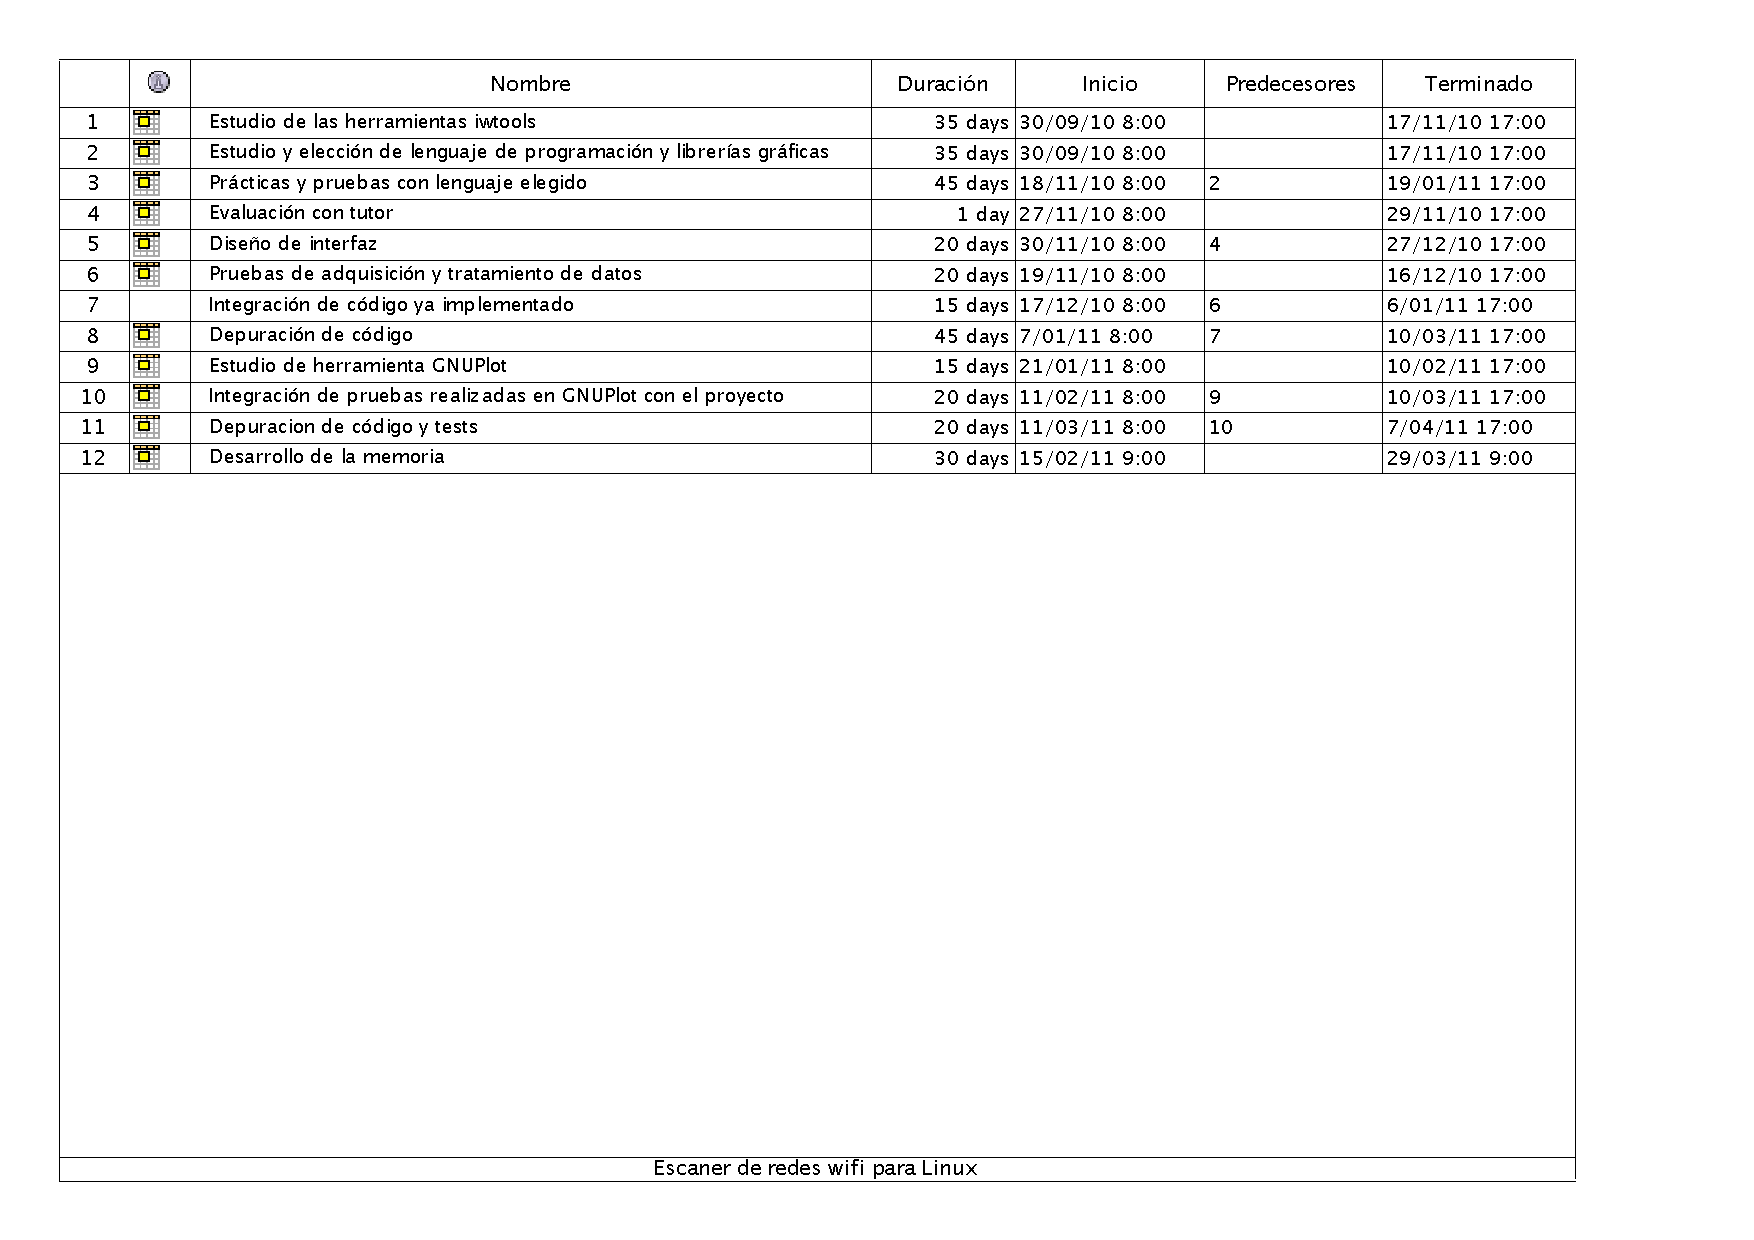
\includepdf[]{src/planificacion_por_hitos.pdf}
 \newpage{\pagestyle{empty}\cleardoublepage} 
    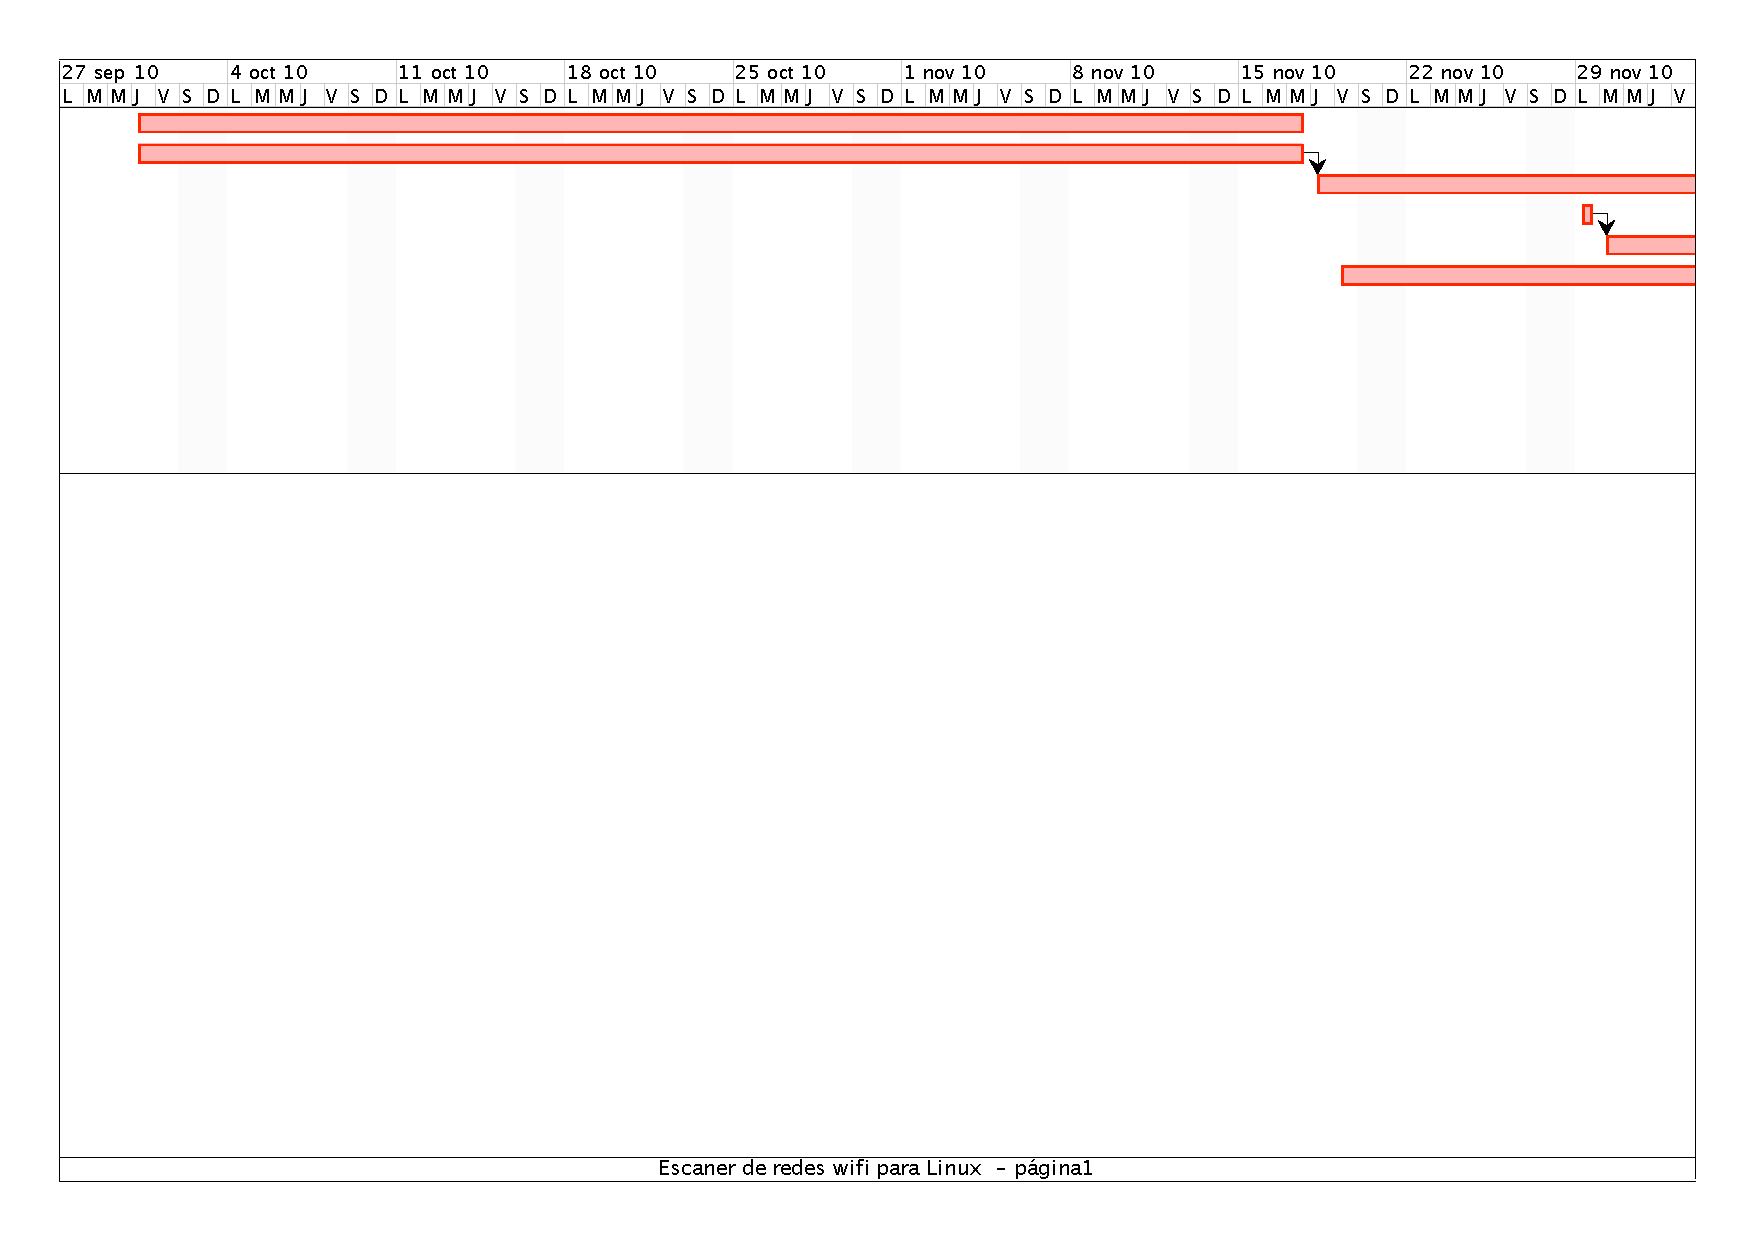
\includepdf[pages={1-3}]{src/planificacion_gantt.pdf}
 \newpage{\pagestyle{empty}\cleardoublepage} 

\section*{Presupuesto}

Tomando �ste proyecto desde cero, la inversi�n a realizar no es muy elevada. A continuaci�n se detallan los costes del desarrollo:\\

\begin{center}
\begin{table}
\begin{tabular}{|c|c|}
\hline \rule[-2ex]{0pt}{5.5ex} \textbf{Elemento} & Precio \\ 
\hline \rule[-2ex]{0pt}{5.5ex} Libro C++ GUI Programming with Qt 4 & prestado en la biblioteca (0 \euro) \\ 
\hline \rule[-2ex]{0pt}{5.5ex} Libro Foundations of Qt Development  & 33\$ \\ 
\hline \rule[-2ex]{0pt}{5.5ex} Herramientas Qt & 0\euro \\ 
\hline \rule[-2ex]{0pt}{5.5ex} Herramientas IwTools & 0\euro \\ 
\hline \rule[-2ex]{0pt}{5.5ex} Gnuplot & 0\euro \\ 
\hline \rule[-2ex]{0pt}{5.5ex} \LaTeX & 0\euro \\ 
\hline \rule[-2ex]{0pt}{5.5ex} Licencia ArchLinux & 0\euro \\ 
\hline \rule[-2ex]{0pt}{5.5ex} total & 33\$ \\ 
\hline 
\end{tabular} 
\caption{Tabla de presupuesto}
\label{Tabla de presupuesto}
\end{table}
\end{center}

\section*{Otros comentarios}
El rastreo y verificaci�n de redes inal�mbricas se ha convertido hoy en una necesidad, al popularizarse el est�ndar IEEE 802.11. Para una correcta transmisi�n de datos es necesario tener en cuenta estos puntos:
\begin{itemize}
	\item Que la se�al del punto de acceso no sea demasiado d�bil.
	\item Que de existir m�s redes inal�mbricas, evitar la solapacion en un mismo canal.
\end{itemize} 
